% Options for packages loaded elsewhere
\PassOptionsToPackage{unicode}{hyperref}
\PassOptionsToPackage{hyphens}{url}
%
\documentclass[
]{article}
\usepackage{amsmath,amssymb}
\usepackage{lmodern}
\usepackage{iftex}
\ifPDFTeX
  \usepackage[T1]{fontenc}
  \usepackage[utf8]{inputenc}
  \usepackage{textcomp} % provide euro and other symbols
\else % if luatex or xetex
  \usepackage{unicode-math}
  \defaultfontfeatures{Scale=MatchLowercase}
  \defaultfontfeatures[\rmfamily]{Ligatures=TeX,Scale=1}
\fi
% Use upquote if available, for straight quotes in verbatim environments
\IfFileExists{upquote.sty}{\usepackage{upquote}}{}
\IfFileExists{microtype.sty}{% use microtype if available
  \usepackage[]{microtype}
  \UseMicrotypeSet[protrusion]{basicmath} % disable protrusion for tt fonts
}{}
\makeatletter
\@ifundefined{KOMAClassName}{% if non-KOMA class
  \IfFileExists{parskip.sty}{%
    \usepackage{parskip}
  }{% else
    \setlength{\parindent}{0pt}
    \setlength{\parskip}{6pt plus 2pt minus 1pt}}
}{% if KOMA class
  \KOMAoptions{parskip=half}}
\makeatother
\usepackage{xcolor}
\usepackage[margin=1in]{geometry}
\usepackage{color}
\usepackage{fancyvrb}
\newcommand{\VerbBar}{|}
\newcommand{\VERB}{\Verb[commandchars=\\\{\}]}
\DefineVerbatimEnvironment{Highlighting}{Verbatim}{commandchars=\\\{\}}
% Add ',fontsize=\small' for more characters per line
\usepackage{framed}
\definecolor{shadecolor}{RGB}{248,248,248}
\newenvironment{Shaded}{\begin{snugshade}}{\end{snugshade}}
\newcommand{\AlertTok}[1]{\textcolor[rgb]{0.94,0.16,0.16}{#1}}
\newcommand{\AnnotationTok}[1]{\textcolor[rgb]{0.56,0.35,0.01}{\textbf{\textit{#1}}}}
\newcommand{\AttributeTok}[1]{\textcolor[rgb]{0.77,0.63,0.00}{#1}}
\newcommand{\BaseNTok}[1]{\textcolor[rgb]{0.00,0.00,0.81}{#1}}
\newcommand{\BuiltInTok}[1]{#1}
\newcommand{\CharTok}[1]{\textcolor[rgb]{0.31,0.60,0.02}{#1}}
\newcommand{\CommentTok}[1]{\textcolor[rgb]{0.56,0.35,0.01}{\textit{#1}}}
\newcommand{\CommentVarTok}[1]{\textcolor[rgb]{0.56,0.35,0.01}{\textbf{\textit{#1}}}}
\newcommand{\ConstantTok}[1]{\textcolor[rgb]{0.00,0.00,0.00}{#1}}
\newcommand{\ControlFlowTok}[1]{\textcolor[rgb]{0.13,0.29,0.53}{\textbf{#1}}}
\newcommand{\DataTypeTok}[1]{\textcolor[rgb]{0.13,0.29,0.53}{#1}}
\newcommand{\DecValTok}[1]{\textcolor[rgb]{0.00,0.00,0.81}{#1}}
\newcommand{\DocumentationTok}[1]{\textcolor[rgb]{0.56,0.35,0.01}{\textbf{\textit{#1}}}}
\newcommand{\ErrorTok}[1]{\textcolor[rgb]{0.64,0.00,0.00}{\textbf{#1}}}
\newcommand{\ExtensionTok}[1]{#1}
\newcommand{\FloatTok}[1]{\textcolor[rgb]{0.00,0.00,0.81}{#1}}
\newcommand{\FunctionTok}[1]{\textcolor[rgb]{0.00,0.00,0.00}{#1}}
\newcommand{\ImportTok}[1]{#1}
\newcommand{\InformationTok}[1]{\textcolor[rgb]{0.56,0.35,0.01}{\textbf{\textit{#1}}}}
\newcommand{\KeywordTok}[1]{\textcolor[rgb]{0.13,0.29,0.53}{\textbf{#1}}}
\newcommand{\NormalTok}[1]{#1}
\newcommand{\OperatorTok}[1]{\textcolor[rgb]{0.81,0.36,0.00}{\textbf{#1}}}
\newcommand{\OtherTok}[1]{\textcolor[rgb]{0.56,0.35,0.01}{#1}}
\newcommand{\PreprocessorTok}[1]{\textcolor[rgb]{0.56,0.35,0.01}{\textit{#1}}}
\newcommand{\RegionMarkerTok}[1]{#1}
\newcommand{\SpecialCharTok}[1]{\textcolor[rgb]{0.00,0.00,0.00}{#1}}
\newcommand{\SpecialStringTok}[1]{\textcolor[rgb]{0.31,0.60,0.02}{#1}}
\newcommand{\StringTok}[1]{\textcolor[rgb]{0.31,0.60,0.02}{#1}}
\newcommand{\VariableTok}[1]{\textcolor[rgb]{0.00,0.00,0.00}{#1}}
\newcommand{\VerbatimStringTok}[1]{\textcolor[rgb]{0.31,0.60,0.02}{#1}}
\newcommand{\WarningTok}[1]{\textcolor[rgb]{0.56,0.35,0.01}{\textbf{\textit{#1}}}}
\usepackage{graphicx}
\makeatletter
\def\maxwidth{\ifdim\Gin@nat@width>\linewidth\linewidth\else\Gin@nat@width\fi}
\def\maxheight{\ifdim\Gin@nat@height>\textheight\textheight\else\Gin@nat@height\fi}
\makeatother
% Scale images if necessary, so that they will not overflow the page
% margins by default, and it is still possible to overwrite the defaults
% using explicit options in \includegraphics[width, height, ...]{}
\setkeys{Gin}{width=\maxwidth,height=\maxheight,keepaspectratio}
% Set default figure placement to htbp
\makeatletter
\def\fps@figure{htbp}
\makeatother
\setlength{\emergencystretch}{3em} % prevent overfull lines
\providecommand{\tightlist}{%
  \setlength{\itemsep}{0pt}\setlength{\parskip}{0pt}}
\setcounter{secnumdepth}{-\maxdimen} % remove section numbering
\ifLuaTeX
  \usepackage{selnolig}  % disable illegal ligatures
\fi
\IfFileExists{bookmark.sty}{\usepackage{bookmark}}{\usepackage{hyperref}}
\IfFileExists{xurl.sty}{\usepackage{xurl}}{} % add URL line breaks if available
\urlstyle{same} % disable monospaced font for URLs
\hypersetup{
  pdftitle={Exercises 1},
  pdfauthor={Cameron Wheatley},
  hidelinks,
  pdfcreator={LaTeX via pandoc}}

\title{Exercises 1}
\author{Cameron Wheatley}
\date{1/29/2023}

\begin{document}
\maketitle

\begin{Shaded}
\begin{Highlighting}[]
\FunctionTok{library}\NormalTok{(readr)}
\NormalTok{ABIA }\OtherTok{\textless{}{-}} \FunctionTok{read\_csv}\NormalTok{(}\StringTok{"https://raw.githubusercontent.com/jgscott/ECO395M/master/data/ABIA.csv"}\NormalTok{)}
\end{Highlighting}
\end{Shaded}

\begin{verbatim}
## Rows: 99260 Columns: 29
## -- Column specification --------------------------------------------------------
## Delimiter: ","
## chr  (5): UniqueCarrier, TailNum, Origin, Dest, CancellationCode
## dbl (24): Year, Month, DayofMonth, DayOfWeek, DepTime, CRSDepTime, ArrTime, ...
## 
## i Use `spec()` to retrieve the full column specification for this data.
## i Specify the column types or set `show_col_types = FALSE` to quiet this message.
\end{verbatim}

\begin{Shaded}
\begin{Highlighting}[]
\FunctionTok{View}\NormalTok{(ABIA)}
\end{Highlighting}
\end{Shaded}

\hypertarget{a-histogram-of-flight-distance-faceted-by-each-day-of-the-week-1monday-7sunday}{%
\section{A histogram of flight distance faceted by each day of the week
(1=Monday,
7=Sunday)}\label{a-histogram-of-flight-distance-faceted-by-each-day-of-the-week-1monday-7sunday}}

\begin{Shaded}
\begin{Highlighting}[]
\FunctionTok{library}\NormalTok{(ggplot2)}
\FunctionTok{library}\NormalTok{(tidyverse)}
\end{Highlighting}
\end{Shaded}

\begin{verbatim}
## -- Attaching packages --------------------------------------- tidyverse 1.3.1 --
\end{verbatim}

\begin{verbatim}
## v tibble  3.1.7     v dplyr   1.0.9
## v tidyr   1.2.0     v stringr 1.4.0
## v purrr   0.3.4     v forcats 0.5.1
\end{verbatim}

\begin{verbatim}
## -- Conflicts ------------------------------------------ tidyverse_conflicts() --
## x dplyr::filter() masks stats::filter()
## x dplyr::lag()    masks stats::lag()
\end{verbatim}

\begin{Shaded}
\begin{Highlighting}[]
\FunctionTok{ggplot}\NormalTok{(}\AttributeTok{data =}\NormalTok{ ABIA) }\SpecialCharTok{+} \FunctionTok{geom\_histogram}\NormalTok{(}\FunctionTok{aes}\NormalTok{(}\AttributeTok{x=}\NormalTok{Distance), }\AttributeTok{binwidth =} \DecValTok{100}\NormalTok{) }\SpecialCharTok{+} \FunctionTok{facet\_wrap}\NormalTok{(}\SpecialCharTok{\textasciitilde{}}\NormalTok{DayOfWeek)}
\end{Highlighting}
\end{Shaded}

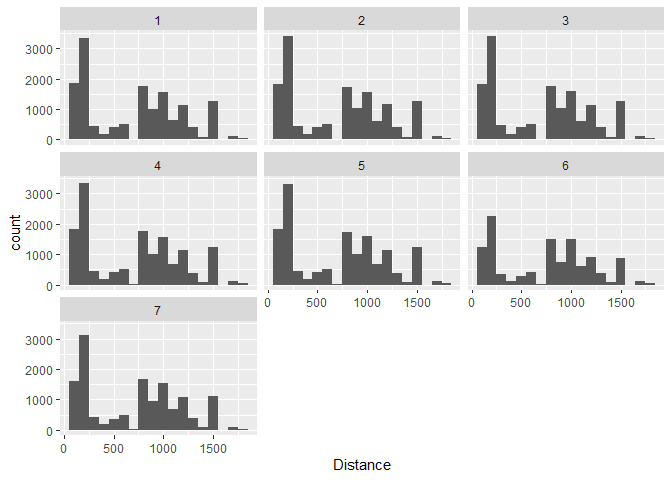
\includegraphics{Homework-1_files/figure-latex/unnamed-chunk-2-1.pdf} \#
While the distribution of flight distance remains similar throughout the
week, the total number of filghts appears to decrease until Sunday.

\begin{Shaded}
\begin{Highlighting}[]
\FunctionTok{library}\NormalTok{(readr)}
\NormalTok{olympics\_top20 }\OtherTok{\textless{}{-}} \FunctionTok{read\_csv}\NormalTok{(}\StringTok{"https://raw.githubusercontent.com/jgscott/ECO395M/master/data/olympics\_top20.csv"}\NormalTok{)}
\end{Highlighting}
\end{Shaded}

\begin{verbatim}
## Rows: 23850 Columns: 15
## -- Column specification --------------------------------------------------------
## Delimiter: ","
## chr (10): name, sex, team, noc, games, season, city, sport, event, medal
## dbl  (5): id, age, height, weight, year
## 
## i Use `spec()` to retrieve the full column specification for this data.
## i Specify the column types or set `show_col_types = FALSE` to quiet this message.
\end{verbatim}

\begin{Shaded}
\begin{Highlighting}[]
\FunctionTok{View}\NormalTok{(olympics\_top20)}
\end{Highlighting}
\end{Shaded}

\hypertarget{part-a-95th-percentile-of-female-heights-across-all-sports-basketball-is-tallest}{%
\section{Part A: 95th percentile of female heights across all sports
(Basketball is
tallest)}\label{part-a-95th-percentile-of-female-heights-across-all-sports-basketball-is-tallest}}

\begin{Shaded}
\begin{Highlighting}[]
\NormalTok{olympics\_heightf }\OtherTok{=}\NormalTok{ olympics\_top20 }\SpecialCharTok{\%\textgreater{}\%}
\FunctionTok{group\_by}\NormalTok{(sex, sport) }\SpecialCharTok{\%\textgreater{}\%}
\FunctionTok{summarize}\NormalTok{(}\AttributeTok{q95\_height =} \FunctionTok{quantile}\NormalTok{(height, }\FloatTok{0.95}\NormalTok{))}
\end{Highlighting}
\end{Shaded}

\begin{verbatim}
## `summarise()` has grouped output by 'sex'. You can override using the `.groups`
## argument.
\end{verbatim}

\hypertarget{part-b-highest-female-variability-in-height-is-10.87-rowing-womens-coexed-fours}{%
\section{Part B: Highest female variability in height is 10.87 (``Rowing
Women's Coexed
Fours'')}\label{part-b-highest-female-variability-in-height-is-10.87-rowing-womens-coexed-fours}}

\begin{Shaded}
\begin{Highlighting}[]
\NormalTok{olympics\_sdf }\OtherTok{=}\NormalTok{ olympics\_top20 }\SpecialCharTok{\%\textgreater{}\%}
\FunctionTok{group\_by}\NormalTok{(sex, event) }\SpecialCharTok{\%\textgreater{}\%}
\FunctionTok{summarize}\NormalTok{(}\AttributeTok{sd\_height =} \FunctionTok{sd}\NormalTok{(height)) }\SpecialCharTok{\%\textgreater{}\%}
\FunctionTok{arrange}\NormalTok{(sd\_height)}
\end{Highlighting}
\end{Shaded}

\begin{verbatim}
## `summarise()` has grouped output by 'sex'. You can override using the `.groups`
## argument.
\end{verbatim}

\hypertarget{part-c-before-women-competed-mean-age-increased-dramatiacally-for-men-then-fell-back-down-to-the-20-25-years-old-interval.-mean-age-for-women-has-remained-slightly-below-men-over-time.}{%
\section{Part C: Before women competed, mean age increased dramatiacally
for men, then fell back down to the 20-25 years old interval. Mean age
for women has remained slightly below men over
time.}\label{part-c-before-women-competed-mean-age-increased-dramatiacally-for-men-then-fell-back-down-to-the-20-25-years-old-interval.-mean-age-for-women-has-remained-slightly-below-men-over-time.}}

\begin{Shaded}
\begin{Highlighting}[]
\NormalTok{olympics\_age }\OtherTok{=}\NormalTok{ olympics\_top20 }\SpecialCharTok{\%\textgreater{}\%}
\FunctionTok{group\_by}\NormalTok{(year, sex) }\SpecialCharTok{\%\textgreater{}\%}
\FunctionTok{filter}\NormalTok{(sport }\SpecialCharTok{==} \StringTok{"Swimming"}\NormalTok{) }\SpecialCharTok{\%\textgreater{}\%}
\FunctionTok{summarize}\NormalTok{(}\AttributeTok{avg\_age =} \FunctionTok{mean}\NormalTok{(age))}
\end{Highlighting}
\end{Shaded}

\begin{verbatim}
## `summarise()` has grouped output by 'year'. You can override using the
## `.groups` argument.
\end{verbatim}

\begin{Shaded}
\begin{Highlighting}[]
\FunctionTok{ggplot}\NormalTok{(}\AttributeTok{data =}\NormalTok{ olympics\_age) }\SpecialCharTok{+} \FunctionTok{geom\_line}\NormalTok{(}\FunctionTok{aes}\NormalTok{(}\AttributeTok{x=}\NormalTok{year, }\AttributeTok{y=}\NormalTok{avg\_age, }\AttributeTok{color=}\NormalTok{sex)) }\SpecialCharTok{+} \FunctionTok{ggtitle}\NormalTok{(}\StringTok{"Mean age of Olympic swimmers over time by sex"}\NormalTok{)}
\end{Highlighting}
\end{Shaded}

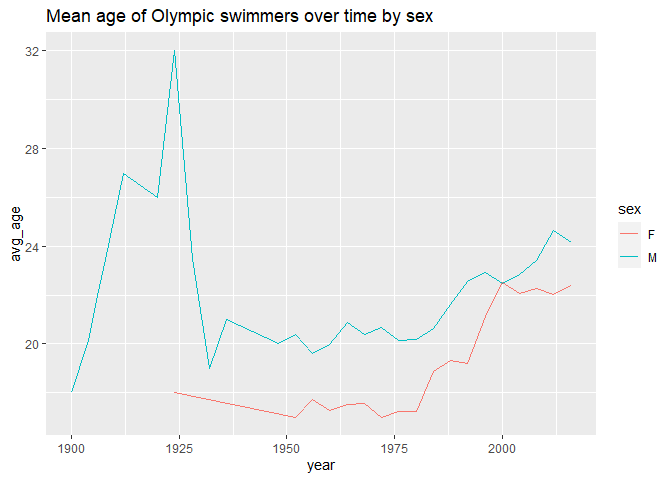
\includegraphics{Homework-1_files/figure-latex/unnamed-chunk-6-1.pdf}

\begin{Shaded}
\begin{Highlighting}[]
\FunctionTok{library}\NormalTok{(readr)}
\NormalTok{sclass }\OtherTok{\textless{}{-}} \FunctionTok{read\_csv}\NormalTok{(}\StringTok{"https://raw.githubusercontent.com/jgscott/ECO395M/master/data/sclass.csv"}\NormalTok{)}
\end{Highlighting}
\end{Shaded}

\begin{verbatim}
## Rows: 29466 Columns: 17
## -- Column specification --------------------------------------------------------
## Delimiter: ","
## chr (11): trim, subTrim, condition, color, displacement, fuel, state, region...
## dbl  (5): id, mileage, year, featureCount, price
## lgl  (1): isOneOwner
## 
## i Use `spec()` to retrieve the full column specification for this data.
## i Specify the column types or set `show_col_types = FALSE` to quiet this message.
\end{verbatim}

\begin{Shaded}
\begin{Highlighting}[]
\FunctionTok{View}\NormalTok{(sclass)}
\end{Highlighting}
\end{Shaded}

\hypertarget{get-two-separate-models-for-both-trims}{%
\section{Get two separate models for both
trims}\label{get-two-separate-models-for-both-trims}}

\begin{Shaded}
\begin{Highlighting}[]
\NormalTok{sclass\_350 }\OtherTok{=}\NormalTok{ sclass }\SpecialCharTok{\%\textgreater{}\%}
\FunctionTok{filter}\NormalTok{(trim }\SpecialCharTok{==} \StringTok{"350"}\NormalTok{)}

\NormalTok{sclass\_65AMG }\OtherTok{=}\NormalTok{ sclass }\SpecialCharTok{\%\textgreater{}\%}
\FunctionTok{filter}\NormalTok{(trim }\SpecialCharTok{==} \StringTok{"65 AMG"}\NormalTok{)}
\end{Highlighting}
\end{Shaded}

\hypertarget{create-train-test-split-for-350-trim-and-find-right-value-for-k-in-knn}{%
\section{Create train test split for 350 trim and find right value for k
in
knn}\label{create-train-test-split-for-350-trim-and-find-right-value-for-k-in-knn}}

\begin{Shaded}
\begin{Highlighting}[]
\FunctionTok{library}\NormalTok{(tidyverse)}
\FunctionTok{library}\NormalTok{(ggplot2)}
\FunctionTok{library}\NormalTok{(rsample)}
\end{Highlighting}
\end{Shaded}

\begin{verbatim}
## Warning: package 'rsample' was built under R version 4.2.2
\end{verbatim}

\begin{Shaded}
\begin{Highlighting}[]
\FunctionTok{library}\NormalTok{(caret)}
\end{Highlighting}
\end{Shaded}

\begin{verbatim}
## Warning: package 'caret' was built under R version 4.2.2
\end{verbatim}

\begin{verbatim}
## Loading required package: lattice
\end{verbatim}

\begin{verbatim}
## 
## Attaching package: 'caret'
\end{verbatim}

\begin{verbatim}
## The following object is masked from 'package:purrr':
## 
##     lift
\end{verbatim}

\begin{Shaded}
\begin{Highlighting}[]
\FunctionTok{library}\NormalTok{(modelr)}
\FunctionTok{library}\NormalTok{(parallel)}
\FunctionTok{library}\NormalTok{(foreach)}
\end{Highlighting}
\end{Shaded}

\begin{verbatim}
## Warning: package 'foreach' was built under R version 4.2.2
\end{verbatim}

\begin{verbatim}
## 
## Attaching package: 'foreach'
\end{verbatim}

\begin{verbatim}
## The following objects are masked from 'package:purrr':
## 
##     accumulate, when
\end{verbatim}

\begin{Shaded}
\begin{Highlighting}[]
\NormalTok{sclass\_350\_split }\OtherTok{=} \FunctionTok{initial\_split}\NormalTok{(sclass\_350, }\AttributeTok{prop=}\FloatTok{0.8}\NormalTok{)}
\NormalTok{sclass\_350\_train }\OtherTok{=} \FunctionTok{training}\NormalTok{(sclass\_350\_split)}
\NormalTok{sclass\_350\_test }\OtherTok{=} \FunctionTok{testing}\NormalTok{(sclass\_350\_split)}

\NormalTok{knn2 }\OtherTok{=} \FunctionTok{knnreg}\NormalTok{(price }\SpecialCharTok{\textasciitilde{}}\NormalTok{ mileage, }\AttributeTok{data=}\NormalTok{sclass\_350\_train, }\AttributeTok{k=}\DecValTok{2}\NormalTok{)}
\FunctionTok{rmse}\NormalTok{(knn2, sclass\_350\_test)}
\end{Highlighting}
\end{Shaded}

\begin{verbatim}
## [1] 11503.38
\end{verbatim}

\begin{Shaded}
\begin{Highlighting}[]
\NormalTok{rmse\_out2 }\OtherTok{=} \FunctionTok{foreach}\NormalTok{(}\AttributeTok{i=}\DecValTok{1}\SpecialCharTok{:}\DecValTok{10}\NormalTok{, }\FunctionTok{combine}\NormalTok{(}\StringTok{\textquotesingle{}c\textquotesingle{}}\NormalTok{)) }\SpecialCharTok{\%do\%}\NormalTok{ \{}
\NormalTok{  sclass\_350\_split }\OtherTok{=} \FunctionTok{initial\_split}\NormalTok{(sclass\_350, }\AttributeTok{prop=}\FloatTok{0.8}\NormalTok{)}
\NormalTok{  sclass\_350\_train }\OtherTok{=} \FunctionTok{training}\NormalTok{(sclass\_350\_split)}
\NormalTok{  sclass\_350\_test }\OtherTok{=} \FunctionTok{testing}\NormalTok{(sclass\_350\_split)}
  
\NormalTok{  knn2 }\OtherTok{=} \FunctionTok{knnreg}\NormalTok{(price }\SpecialCharTok{\textasciitilde{}}\NormalTok{ mileage, }\AttributeTok{data=}\NormalTok{sclass\_350\_train, }\AttributeTok{k=}\DecValTok{2}\NormalTok{)}
  \FunctionTok{rmse}\NormalTok{(knn2, sclass\_350\_test)}
\NormalTok{\}}
\end{Highlighting}
\end{Shaded}

\begin{verbatim}
## Warning: `combine()` was deprecated in dplyr 1.0.0.
## i Please use `vctrs::vec_c()` instead.
\end{verbatim}

\begin{Shaded}
\begin{Highlighting}[]
\NormalTok{knn5 }\OtherTok{=} \FunctionTok{knnreg}\NormalTok{(price }\SpecialCharTok{\textasciitilde{}}\NormalTok{ mileage, }\AttributeTok{data=}\NormalTok{sclass\_350\_train, }\AttributeTok{k=}\DecValTok{5}\NormalTok{)}
\FunctionTok{rmse}\NormalTok{(knn5, sclass\_350\_test)}
\end{Highlighting}
\end{Shaded}

\begin{verbatim}
## [1] 11233.37
\end{verbatim}

\begin{Shaded}
\begin{Highlighting}[]
\NormalTok{rmse\_out5 }\OtherTok{=} \FunctionTok{foreach}\NormalTok{(}\AttributeTok{i=}\DecValTok{1}\SpecialCharTok{:}\DecValTok{10}\NormalTok{, }\FunctionTok{combine}\NormalTok{(}\StringTok{\textquotesingle{}c\textquotesingle{}}\NormalTok{)) }\SpecialCharTok{\%do\%}\NormalTok{ \{}
\NormalTok{  sclass\_350\_split }\OtherTok{=} \FunctionTok{initial\_split}\NormalTok{(sclass\_350, }\AttributeTok{prop=}\FloatTok{0.8}\NormalTok{)}
\NormalTok{  sclass\_350\_train }\OtherTok{=} \FunctionTok{training}\NormalTok{(sclass\_350\_split)}
\NormalTok{  sclass\_350\_test }\OtherTok{=} \FunctionTok{testing}\NormalTok{(sclass\_350\_split)}
  
\NormalTok{  knn5 }\OtherTok{=} \FunctionTok{knnreg}\NormalTok{(price }\SpecialCharTok{\textasciitilde{}}\NormalTok{ mileage, }\AttributeTok{data=}\NormalTok{sclass\_350\_train, }\AttributeTok{k=}\DecValTok{5}\NormalTok{)}
  \FunctionTok{rmse}\NormalTok{(knn5, sclass\_350\_test)}
\NormalTok{\}}

\NormalTok{knn10 }\OtherTok{=} \FunctionTok{knnreg}\NormalTok{(price }\SpecialCharTok{\textasciitilde{}}\NormalTok{ mileage, }\AttributeTok{data=}\NormalTok{sclass\_350\_train, }\AttributeTok{k=}\DecValTok{10}\NormalTok{)}
\FunctionTok{rmse}\NormalTok{(knn10, sclass\_350\_test)}
\end{Highlighting}
\end{Shaded}

\begin{verbatim}
## [1] 9242.442
\end{verbatim}

\begin{Shaded}
\begin{Highlighting}[]
\NormalTok{rmse\_out10 }\OtherTok{=} \FunctionTok{foreach}\NormalTok{(}\AttributeTok{i=}\DecValTok{1}\SpecialCharTok{:}\DecValTok{10}\NormalTok{, }\FunctionTok{combine}\NormalTok{(}\StringTok{\textquotesingle{}c\textquotesingle{}}\NormalTok{)) }\SpecialCharTok{\%do\%}\NormalTok{ \{}
\NormalTok{  sclass\_350\_split }\OtherTok{=} \FunctionTok{initial\_split}\NormalTok{(sclass\_350, }\AttributeTok{prop=}\FloatTok{0.8}\NormalTok{)}
\NormalTok{  sclass\_350\_train }\OtherTok{=} \FunctionTok{training}\NormalTok{(sclass\_350\_split)}
\NormalTok{  sclass\_350\_test }\OtherTok{=} \FunctionTok{testing}\NormalTok{(sclass\_350\_split)}
  
\NormalTok{  knn10 }\OtherTok{=} \FunctionTok{knnreg}\NormalTok{(price }\SpecialCharTok{\textasciitilde{}}\NormalTok{ mileage, }\AttributeTok{data=}\NormalTok{sclass\_350\_train, }\AttributeTok{k=}\DecValTok{10}\NormalTok{)}
  \FunctionTok{rmse}\NormalTok{(knn10, sclass\_350\_test)}
\NormalTok{\}}

\NormalTok{knn20 }\OtherTok{=} \FunctionTok{knnreg}\NormalTok{(price }\SpecialCharTok{\textasciitilde{}}\NormalTok{ mileage, }\AttributeTok{data=}\NormalTok{sclass\_350\_train, }\AttributeTok{k=}\DecValTok{20}\NormalTok{)}
\FunctionTok{rmse}\NormalTok{(knn20, sclass\_350\_test)}
\end{Highlighting}
\end{Shaded}

\begin{verbatim}
## [1] 9901.261
\end{verbatim}

\begin{Shaded}
\begin{Highlighting}[]
\NormalTok{rmse\_out20 }\OtherTok{=} \FunctionTok{foreach}\NormalTok{(}\AttributeTok{i=}\DecValTok{1}\SpecialCharTok{:}\DecValTok{10}\NormalTok{, }\FunctionTok{combine}\NormalTok{(}\StringTok{\textquotesingle{}c\textquotesingle{}}\NormalTok{)) }\SpecialCharTok{\%do\%}\NormalTok{ \{}
\NormalTok{  sclass\_350\_split }\OtherTok{=} \FunctionTok{initial\_split}\NormalTok{(sclass\_350, }\AttributeTok{prop=}\FloatTok{0.8}\NormalTok{)}
\NormalTok{  sclass\_350\_train }\OtherTok{=} \FunctionTok{training}\NormalTok{(sclass\_350\_split)}
\NormalTok{  sclass\_350\_test }\OtherTok{=} \FunctionTok{testing}\NormalTok{(sclass\_350\_split)}
  
\NormalTok{  knn20 }\OtherTok{=} \FunctionTok{knnreg}\NormalTok{(price }\SpecialCharTok{\textasciitilde{}}\NormalTok{ mileage, }\AttributeTok{data=}\NormalTok{sclass\_350\_train, }\AttributeTok{k=}\DecValTok{20}\NormalTok{)}
  \FunctionTok{rmse}\NormalTok{(knn20, sclass\_350\_test)}
\NormalTok{\}}

\NormalTok{knn25 }\OtherTok{=} \FunctionTok{knnreg}\NormalTok{(price }\SpecialCharTok{\textasciitilde{}}\NormalTok{ mileage, }\AttributeTok{data=}\NormalTok{sclass\_350\_train, }\AttributeTok{k=}\DecValTok{25}\NormalTok{)}
\FunctionTok{rmse}\NormalTok{(knn25, sclass\_350\_test)}
\end{Highlighting}
\end{Shaded}

\begin{verbatim}
## [1] 10292.9
\end{verbatim}

\begin{Shaded}
\begin{Highlighting}[]
\NormalTok{rmse\_out25 }\OtherTok{=} \FunctionTok{foreach}\NormalTok{(}\AttributeTok{i=}\DecValTok{1}\SpecialCharTok{:}\DecValTok{10}\NormalTok{, }\FunctionTok{combine}\NormalTok{(}\StringTok{\textquotesingle{}c\textquotesingle{}}\NormalTok{)) }\SpecialCharTok{\%do\%}\NormalTok{ \{}
\NormalTok{  sclass\_350\_split }\OtherTok{=} \FunctionTok{initial\_split}\NormalTok{(sclass\_350, }\AttributeTok{prop=}\FloatTok{0.8}\NormalTok{)}
\NormalTok{  sclass\_350\_train }\OtherTok{=} \FunctionTok{training}\NormalTok{(sclass\_350\_split)}
\NormalTok{  sclass\_350\_test }\OtherTok{=} \FunctionTok{testing}\NormalTok{(sclass\_350\_split)}
  
\NormalTok{  knn25 }\OtherTok{=} \FunctionTok{knnreg}\NormalTok{(price }\SpecialCharTok{\textasciitilde{}}\NormalTok{ mileage, }\AttributeTok{data=}\NormalTok{sclass\_350\_train, }\AttributeTok{k=}\DecValTok{25}\NormalTok{)}
  \FunctionTok{rmse}\NormalTok{(knn25, sclass\_350\_test)}
\NormalTok{\}}

\NormalTok{knn30 }\OtherTok{=} \FunctionTok{knnreg}\NormalTok{(price }\SpecialCharTok{\textasciitilde{}}\NormalTok{ mileage, }\AttributeTok{data=}\NormalTok{sclass\_350\_train, }\AttributeTok{k=}\DecValTok{30}\NormalTok{)}
\FunctionTok{rmse}\NormalTok{(knn30, sclass\_350\_test)}
\end{Highlighting}
\end{Shaded}

\begin{verbatim}
## [1] 8235.539
\end{verbatim}

\begin{Shaded}
\begin{Highlighting}[]
\NormalTok{rmse\_out30 }\OtherTok{=} \FunctionTok{foreach}\NormalTok{(}\AttributeTok{i=}\DecValTok{1}\SpecialCharTok{:}\DecValTok{10}\NormalTok{, }\FunctionTok{combine}\NormalTok{(}\StringTok{\textquotesingle{}c\textquotesingle{}}\NormalTok{)) }\SpecialCharTok{\%do\%}\NormalTok{ \{}
\NormalTok{  sclass\_350\_split }\OtherTok{=} \FunctionTok{initial\_split}\NormalTok{(sclass\_350, }\AttributeTok{prop=}\FloatTok{0.8}\NormalTok{)}
\NormalTok{  sclass\_350\_train }\OtherTok{=} \FunctionTok{training}\NormalTok{(sclass\_350\_split)}
\NormalTok{  sclass\_350\_test }\OtherTok{=} \FunctionTok{testing}\NormalTok{(sclass\_350\_split)}
  
\NormalTok{  knn30 }\OtherTok{=} \FunctionTok{knnreg}\NormalTok{(price }\SpecialCharTok{\textasciitilde{}}\NormalTok{ mileage, }\AttributeTok{data=}\NormalTok{sclass\_350\_train, }\AttributeTok{k=}\DecValTok{30}\NormalTok{)}
  \FunctionTok{rmse}\NormalTok{(knn30, sclass\_350\_test)}
\NormalTok{\}}

\NormalTok{knn35 }\OtherTok{=} \FunctionTok{knnreg}\NormalTok{(price }\SpecialCharTok{\textasciitilde{}}\NormalTok{ mileage, }\AttributeTok{data=}\NormalTok{sclass\_350\_train, }\AttributeTok{k=}\DecValTok{35}\NormalTok{)}
\FunctionTok{rmse}\NormalTok{(knn35, sclass\_350\_test)}
\end{Highlighting}
\end{Shaded}

\begin{verbatim}
## [1] 10227.09
\end{verbatim}

\begin{Shaded}
\begin{Highlighting}[]
\NormalTok{rmse\_out35 }\OtherTok{=} \FunctionTok{foreach}\NormalTok{(}\AttributeTok{i=}\DecValTok{1}\SpecialCharTok{:}\DecValTok{10}\NormalTok{, }\FunctionTok{combine}\NormalTok{(}\StringTok{\textquotesingle{}c\textquotesingle{}}\NormalTok{)) }\SpecialCharTok{\%do\%}\NormalTok{ \{}
\NormalTok{  sclass\_350\_split }\OtherTok{=} \FunctionTok{initial\_split}\NormalTok{(sclass\_350, }\AttributeTok{prop=}\FloatTok{0.8}\NormalTok{)}
\NormalTok{  sclass\_350\_train }\OtherTok{=} \FunctionTok{training}\NormalTok{(sclass\_350\_split)}
\NormalTok{  sclass\_350\_test }\OtherTok{=} \FunctionTok{testing}\NormalTok{(sclass\_350\_split)}
  
\NormalTok{  knn35 }\OtherTok{=} \FunctionTok{knnreg}\NormalTok{(price }\SpecialCharTok{\textasciitilde{}}\NormalTok{ mileage, }\AttributeTok{data=}\NormalTok{sclass\_350\_train, }\AttributeTok{k=}\DecValTok{35}\NormalTok{)}
  \FunctionTok{rmse}\NormalTok{(knn35, sclass\_350\_test)}
\NormalTok{\}}

\NormalTok{knn40 }\OtherTok{=} \FunctionTok{knnreg}\NormalTok{(price }\SpecialCharTok{\textasciitilde{}}\NormalTok{ mileage, }\AttributeTok{data=}\NormalTok{sclass\_350\_train, }\AttributeTok{k=}\DecValTok{40}\NormalTok{)}
\FunctionTok{rmse}\NormalTok{(knn40, sclass\_350\_test)}
\end{Highlighting}
\end{Shaded}

\begin{verbatim}
## [1] 10376.49
\end{verbatim}

\begin{Shaded}
\begin{Highlighting}[]
\NormalTok{rmse\_out40 }\OtherTok{=} \FunctionTok{foreach}\NormalTok{(}\AttributeTok{i=}\DecValTok{1}\SpecialCharTok{:}\DecValTok{10}\NormalTok{, }\FunctionTok{combine}\NormalTok{(}\StringTok{\textquotesingle{}c\textquotesingle{}}\NormalTok{)) }\SpecialCharTok{\%do\%}\NormalTok{ \{}
\NormalTok{  sclass\_350\_split }\OtherTok{=} \FunctionTok{initial\_split}\NormalTok{(sclass\_350, }\AttributeTok{prop=}\FloatTok{0.8}\NormalTok{)}
\NormalTok{  sclass\_350\_train }\OtherTok{=} \FunctionTok{training}\NormalTok{(sclass\_350\_split)}
\NormalTok{  sclass\_350\_test }\OtherTok{=} \FunctionTok{testing}\NormalTok{(sclass\_350\_split)}
  
\NormalTok{  knn40 }\OtherTok{=} \FunctionTok{knnreg}\NormalTok{(price }\SpecialCharTok{\textasciitilde{}}\NormalTok{ mileage, }\AttributeTok{data=}\NormalTok{sclass\_350\_train, }\AttributeTok{k=}\DecValTok{40}\NormalTok{)}
  \FunctionTok{rmse}\NormalTok{(knn40, sclass\_350\_test)}
\NormalTok{\}}
\end{Highlighting}
\end{Shaded}

\hypertarget{run-k-fold-cross-validation-to-plot-rmse-vs.-k}{%
\section{Run k-fold cross-validation to plot RMSE
vs.~k}\label{run-k-fold-cross-validation-to-plot-rmse-vs.-k}}

\begin{Shaded}
\begin{Highlighting}[]
\NormalTok{K\_folds }\OtherTok{=} \DecValTok{5}
\NormalTok{sclass\_350 }\OtherTok{=}\NormalTok{ sclass\_350 }\SpecialCharTok{\%\textgreater{}\%}
  \FunctionTok{mutate}\NormalTok{(}\AttributeTok{fold\_id =} \FunctionTok{rep}\NormalTok{(}\DecValTok{1}\SpecialCharTok{:}\NormalTok{K\_folds, }\AttributeTok{length =} \FunctionTok{nrow}\NormalTok{(sclass\_350)) }\SpecialCharTok{\%\textgreater{}\%}\NormalTok{ sample)}

\FunctionTok{head}\NormalTok{(sclass\_350)}
\end{Highlighting}
\end{Shaded}

\begin{verbatim}
## # A tibble: 6 x 18
##      id trim  subTrim condition isOneOwner mileage  year color  displacement
##   <dbl> <chr> <chr>   <chr>     <lgl>        <dbl> <dbl> <chr>  <chr>       
## 1   282 350   unsp    CPO       FALSE        21929  2012 Black  3.0 L       
## 2   284 350   unsp    CPO       FALSE        17770  2012 Silver 3.0 L       
## 3   285 350   unsp    Used      FALSE        29108  2012 Black  3.0 L       
## 4   288 350   unsp    CPO       FALSE        35004  2013 White  3.0 L       
## 5   289 350   unsp    Used      TRUE         66689  2012 Black  3.0 L       
## 6   290 350   unsp    CPO       FALSE        19567  2012 Black  3.0 L       
## # ... with 9 more variables: fuel <chr>, state <chr>, region <chr>,
## #   soundSystem <chr>, wheelType <chr>, wheelSize <chr>, featureCount <dbl>,
## #   price <dbl>, fold_id <int>
\end{verbatim}

\begin{Shaded}
\begin{Highlighting}[]
\NormalTok{rmse\_cv }\OtherTok{=} \FunctionTok{foreach}\NormalTok{(}\AttributeTok{fold =} \DecValTok{1}\SpecialCharTok{:}\NormalTok{K\_folds, }\AttributeTok{.combine =} \StringTok{\textquotesingle{}c\textquotesingle{}}\NormalTok{) }\SpecialCharTok{\%do\%}\NormalTok{ \{}
\NormalTok{  knn35 }\OtherTok{=} \FunctionTok{knnreg}\NormalTok{(price }\SpecialCharTok{\textasciitilde{}}\NormalTok{ mileage, }\AttributeTok{data=}\FunctionTok{filter}\NormalTok{(sclass\_350, fold\_id }\SpecialCharTok{!=}\NormalTok{ fold), }\AttributeTok{k=}\DecValTok{35}\NormalTok{)}
\NormalTok{  modelr}\SpecialCharTok{::}\FunctionTok{rmse}\NormalTok{(knn35, }\AttributeTok{data=}\FunctionTok{filter}\NormalTok{(sclass\_350, fold\_id }\SpecialCharTok{==}\NormalTok{ fold))}
\NormalTok{\}}

\NormalTok{rmse\_cv}
\end{Highlighting}
\end{Shaded}

\begin{verbatim}
## [1]  9569.643 11188.313  8739.655 11070.818 10683.416
\end{verbatim}

\begin{Shaded}
\begin{Highlighting}[]
\FunctionTok{mean}\NormalTok{(rmse\_cv)}
\end{Highlighting}
\end{Shaded}

\begin{verbatim}
## [1] 10250.37
\end{verbatim}

\begin{Shaded}
\begin{Highlighting}[]
\FunctionTok{sd}\NormalTok{(rmse\_cv)}\SpecialCharTok{/}\FunctionTok{sqrt}\NormalTok{(K\_folds)}
\end{Highlighting}
\end{Shaded}

\begin{verbatim}
## [1] 473.6058
\end{verbatim}

\begin{Shaded}
\begin{Highlighting}[]
\NormalTok{sclass350\_folds }\OtherTok{=} \FunctionTok{crossv\_kfold}\NormalTok{(sclass\_350, }\AttributeTok{k=}\NormalTok{K\_folds)}
\NormalTok{models }\OtherTok{=} \FunctionTok{map}\NormalTok{(sclass350\_folds}\SpecialCharTok{$}\NormalTok{train, }\SpecialCharTok{\textasciitilde{}} \FunctionTok{knnreg}\NormalTok{(price }\SpecialCharTok{\textasciitilde{}}\NormalTok{ mileage, }\AttributeTok{k=}\DecValTok{35}\NormalTok{, }\AttributeTok{data =}\NormalTok{ ., }\AttributeTok{use.all=}\ConstantTok{FALSE}\NormalTok{))}

\NormalTok{errs }\OtherTok{=} \FunctionTok{map2\_dbl}\NormalTok{(models, sclass350\_folds}\SpecialCharTok{$}\NormalTok{test, modelr}\SpecialCharTok{::}\NormalTok{rmse)}

\FunctionTok{mean}\NormalTok{(errs)}
\end{Highlighting}
\end{Shaded}

\begin{verbatim}
## [1] 10075.4
\end{verbatim}

\begin{Shaded}
\begin{Highlighting}[]
\FunctionTok{sd}\NormalTok{(errs)}\SpecialCharTok{/}\FunctionTok{sqrt}\NormalTok{(K\_folds)}
\end{Highlighting}
\end{Shaded}

\begin{verbatim}
## [1] 383.7049
\end{verbatim}

\begin{Shaded}
\begin{Highlighting}[]
\NormalTok{k\_grid }\OtherTok{=} \FunctionTok{c}\NormalTok{(}\DecValTok{2}\NormalTok{, }\DecValTok{4}\NormalTok{, }\DecValTok{6}\NormalTok{, }\DecValTok{8}\NormalTok{, }\DecValTok{10}\NormalTok{, }\DecValTok{15}\NormalTok{, }\DecValTok{20}\NormalTok{, }\DecValTok{25}\NormalTok{, }\DecValTok{30}\NormalTok{, }\DecValTok{35}\NormalTok{, }\DecValTok{40}\NormalTok{, }\DecValTok{45}\NormalTok{, }\DecValTok{50}\NormalTok{, }\DecValTok{60}\NormalTok{, }\DecValTok{70}\NormalTok{, }\DecValTok{80}\NormalTok{, }\DecValTok{90}\NormalTok{, }\DecValTok{100}\NormalTok{, }\DecValTok{125}\NormalTok{, }\DecValTok{150}\NormalTok{, }\DecValTok{175}\NormalTok{, }\DecValTok{200}\NormalTok{, }\DecValTok{250}\NormalTok{, }\DecValTok{300}\NormalTok{)}

\NormalTok{cv\_grid }\OtherTok{=} \FunctionTok{foreach}\NormalTok{(}\AttributeTok{k =}\NormalTok{ k\_grid, }\AttributeTok{.combine=}\StringTok{\textquotesingle{}rbind\textquotesingle{}}\NormalTok{) }\SpecialCharTok{\%dopar\%}\NormalTok{ \{}
\NormalTok{  models }\OtherTok{=} \FunctionTok{map}\NormalTok{(sclass350\_folds}\SpecialCharTok{$}\NormalTok{train, }\SpecialCharTok{\textasciitilde{}} \FunctionTok{knnreg}\NormalTok{(price }\SpecialCharTok{\textasciitilde{}}\NormalTok{ mileage, }\AttributeTok{k=}\NormalTok{k, }\AttributeTok{data =}\NormalTok{ ., }\AttributeTok{use.all=}\ConstantTok{FALSE}\NormalTok{))}
\NormalTok{  errs }\OtherTok{=} \FunctionTok{map2\_dbl}\NormalTok{(models, sclass350\_folds}\SpecialCharTok{$}\NormalTok{test, modelr}\SpecialCharTok{::}\NormalTok{rmse)}
  \FunctionTok{c}\NormalTok{(}\AttributeTok{k=}\NormalTok{k, }\AttributeTok{err =} \FunctionTok{mean}\NormalTok{(errs), }\AttributeTok{std\_err =} \FunctionTok{sd}\NormalTok{(errs)}\SpecialCharTok{/}\FunctionTok{sqrt}\NormalTok{(K\_folds))}
\NormalTok{\} }\SpecialCharTok{\%\textgreater{}\%}\NormalTok{ as.data.frame}
\end{Highlighting}
\end{Shaded}

\begin{verbatim}
## Warning: executing %dopar% sequentially: no parallel backend registered
\end{verbatim}

\begin{Shaded}
\begin{Highlighting}[]
\FunctionTok{head}\NormalTok{(cv\_grid)}
\end{Highlighting}
\end{Shaded}

\begin{verbatim}
##           k       err  std_err
## result.1  2 11419.575 192.0480
## result.2  4 10565.096 411.9735
## result.3  6 10104.164 361.4572
## result.4  8 10046.709 406.5537
## result.5 10  9829.693 436.5004
## result.6 15  9767.796 507.7052
\end{verbatim}

\begin{Shaded}
\begin{Highlighting}[]
\FunctionTok{ggplot}\NormalTok{(cv\_grid) }\SpecialCharTok{+} \FunctionTok{geom\_point}\NormalTok{(}\FunctionTok{aes}\NormalTok{(}\AttributeTok{x=}\NormalTok{k, }\AttributeTok{y=}\NormalTok{err)) }\SpecialCharTok{+} \FunctionTok{geom\_errorbar}\NormalTok{(}\FunctionTok{aes}\NormalTok{(}\AttributeTok{x=}\NormalTok{k, }\AttributeTok{ymin =}\NormalTok{ err}\SpecialCharTok{{-}}\NormalTok{std\_err, }\AttributeTok{ymax =}\NormalTok{ err}\SpecialCharTok{+}\NormalTok{std\_err)) }\SpecialCharTok{+} \FunctionTok{scale\_x\_log10}\NormalTok{()}
\end{Highlighting}
\end{Shaded}

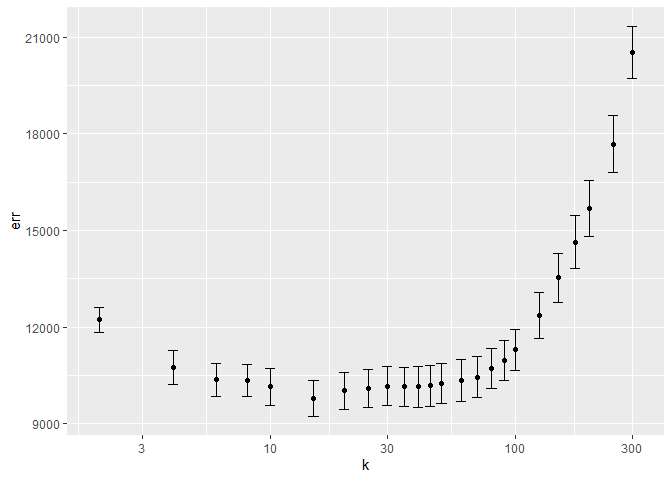
\includegraphics{Homework-1_files/figure-latex/unnamed-chunk-10-1.pdf}
\# Plot the fitted model of price (k=35) vs.~x

\begin{Shaded}
\begin{Highlighting}[]
\NormalTok{sclass\_350\_test }\OtherTok{=}\NormalTok{ sclass\_350\_test }\SpecialCharTok{\%\textgreater{}\%}
  \FunctionTok{mutate}\NormalTok{(}\AttributeTok{price\_pred =} \FunctionTok{predict}\NormalTok{(knn35, sclass\_350\_test))}

\NormalTok{p\_test }\OtherTok{=} \FunctionTok{ggplot}\NormalTok{(}\AttributeTok{data =}\NormalTok{ sclass\_350\_test) }\SpecialCharTok{+} \FunctionTok{geom\_point}\NormalTok{(}\AttributeTok{mapping =} \FunctionTok{aes}\NormalTok{(}\AttributeTok{x=}\NormalTok{mileage, }\AttributeTok{y=}\NormalTok{price), }\AttributeTok{alpha =} \FloatTok{0.2}\NormalTok{) }\SpecialCharTok{+} \FunctionTok{ylim}\NormalTok{(}\DecValTok{7000}\NormalTok{, }\DecValTok{20000}\NormalTok{)}
\NormalTok{p\_test}
\end{Highlighting}
\end{Shaded}

\begin{verbatim}
## Warning: Removed 61 rows containing missing values (geom_point).
\end{verbatim}

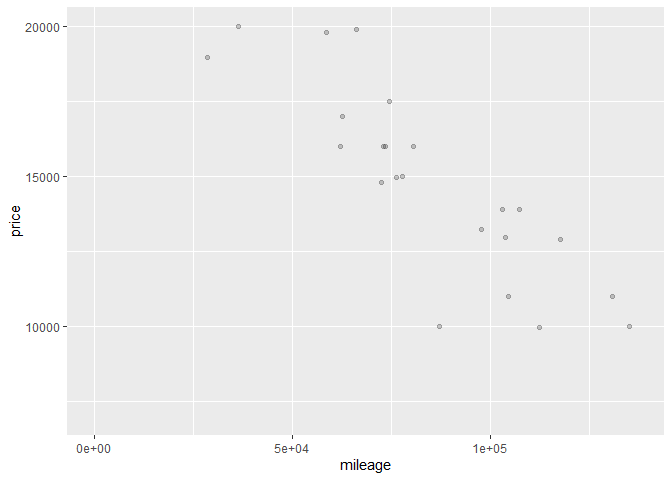
\includegraphics{Homework-1_files/figure-latex/unnamed-chunk-11-1.pdf}

\begin{Shaded}
\begin{Highlighting}[]
\NormalTok{p\_test }\SpecialCharTok{+} \FunctionTok{geom\_line}\NormalTok{(}\FunctionTok{aes}\NormalTok{(}\AttributeTok{x=}\NormalTok{mileage, }\AttributeTok{y=}\NormalTok{price\_pred), }\AttributeTok{color=}\StringTok{\textquotesingle{}green\textquotesingle{}}\NormalTok{, }\AttributeTok{size=}\FloatTok{1.5}\NormalTok{)}
\end{Highlighting}
\end{Shaded}

\begin{verbatim}
## Warning: Removed 61 rows containing missing values (geom_point).
\end{verbatim}

\begin{verbatim}
## Warning: Removed 63 row(s) containing missing values (geom_path).
\end{verbatim}

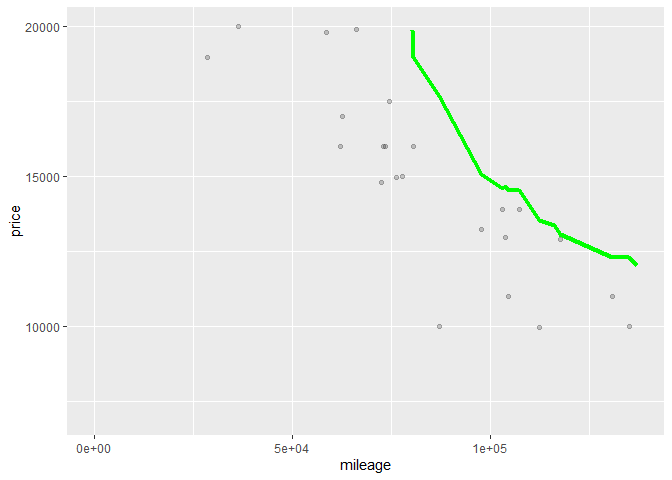
\includegraphics{Homework-1_files/figure-latex/unnamed-chunk-11-2.pdf}

\hypertarget{run-the-same-process-for-the-65-amg-trim-k13}{%
\section{Run the same process for the ``65 AMG'' trim
(k=13)}\label{run-the-same-process-for-the-65-amg-trim-k13}}

\begin{Shaded}
\begin{Highlighting}[]
\NormalTok{sclass\_65AMG\_split }\OtherTok{=} \FunctionTok{initial\_split}\NormalTok{(sclass\_350, }\AttributeTok{prop=}\FloatTok{0.8}\NormalTok{)}
\NormalTok{sclass\_65AMG\_train }\OtherTok{=} \FunctionTok{training}\NormalTok{(sclass\_350\_split)}
\NormalTok{sclass\_65AMG\_test }\OtherTok{=} \FunctionTok{testing}\NormalTok{(sclass\_350\_split)}

\NormalTok{knn2 }\OtherTok{=} \FunctionTok{knnreg}\NormalTok{(price }\SpecialCharTok{\textasciitilde{}}\NormalTok{ mileage, }\AttributeTok{data=}\NormalTok{sclass\_65AMG\_train, }\AttributeTok{k=}\DecValTok{2}\NormalTok{)}
\FunctionTok{rmse}\NormalTok{(knn2, sclass\_65AMG\_test)}
\end{Highlighting}
\end{Shaded}

\begin{verbatim}
## [1] 14318.02
\end{verbatim}

\begin{Shaded}
\begin{Highlighting}[]
\NormalTok{rmse\_out2 }\OtherTok{=} \FunctionTok{foreach}\NormalTok{(}\AttributeTok{i=}\DecValTok{1}\SpecialCharTok{:}\DecValTok{10}\NormalTok{, }\FunctionTok{combine}\NormalTok{(}\StringTok{\textquotesingle{}c\textquotesingle{}}\NormalTok{)) }\SpecialCharTok{\%do\%}\NormalTok{ \{}
\NormalTok{  sclass\_65AMG\_split }\OtherTok{=} \FunctionTok{initial\_split}\NormalTok{(sclass\_65AMG, }\AttributeTok{prop=}\FloatTok{0.8}\NormalTok{)}
\NormalTok{  sclass\_65AMG\_train }\OtherTok{=} \FunctionTok{training}\NormalTok{(sclass\_65AMG\_split)}
\NormalTok{  sclass\_65AMG\_test }\OtherTok{=} \FunctionTok{testing}\NormalTok{(sclass\_65AMG\_split)}
  
\NormalTok{  knn2 }\OtherTok{=} \FunctionTok{knnreg}\NormalTok{(price }\SpecialCharTok{\textasciitilde{}}\NormalTok{ mileage, }\AttributeTok{data=}\NormalTok{sclass\_65AMG\_train, }\AttributeTok{k=}\DecValTok{2}\NormalTok{)}
  \FunctionTok{rmse}\NormalTok{(knn2, sclass\_65AMG\_test)}
\NormalTok{\}}

\NormalTok{knn15 }\OtherTok{=} \FunctionTok{knnreg}\NormalTok{(price }\SpecialCharTok{\textasciitilde{}}\NormalTok{ mileage, }\AttributeTok{data=}\NormalTok{sclass\_65AMG\_train, }\AttributeTok{k=}\DecValTok{15}\NormalTok{)}
\FunctionTok{rmse}\NormalTok{(knn15, sclass\_65AMG\_test)}
\end{Highlighting}
\end{Shaded}

\begin{verbatim}
## [1] 20474.89
\end{verbatim}

\begin{Shaded}
\begin{Highlighting}[]
\NormalTok{rmse\_out15 }\OtherTok{=} \FunctionTok{foreach}\NormalTok{(}\AttributeTok{i=}\DecValTok{1}\SpecialCharTok{:}\DecValTok{10}\NormalTok{, }\FunctionTok{combine}\NormalTok{(}\StringTok{\textquotesingle{}c\textquotesingle{}}\NormalTok{)) }\SpecialCharTok{\%do\%}\NormalTok{ \{}
\NormalTok{  sclass\_65AMG\_split }\OtherTok{=} \FunctionTok{initial\_split}\NormalTok{(sclass\_65AMG, }\AttributeTok{prop=}\FloatTok{0.8}\NormalTok{)}
\NormalTok{  sclass\_65AMG\_train }\OtherTok{=} \FunctionTok{training}\NormalTok{(sclass\_65AMG\_split)}
\NormalTok{  sclass\_65AMG\_test }\OtherTok{=} \FunctionTok{testing}\NormalTok{(sclass\_65AMG\_split)}
  
\NormalTok{  knn15 }\OtherTok{=} \FunctionTok{knnreg}\NormalTok{(price }\SpecialCharTok{\textasciitilde{}}\NormalTok{ mileage, }\AttributeTok{data=}\NormalTok{sclass\_65AMG\_train, }\AttributeTok{k=}\DecValTok{15}\NormalTok{)}
  \FunctionTok{rmse}\NormalTok{(knn15, sclass\_65AMG\_test)}
\NormalTok{\}}

\NormalTok{knn25 }\OtherTok{=} \FunctionTok{knnreg}\NormalTok{(price }\SpecialCharTok{\textasciitilde{}}\NormalTok{ mileage, }\AttributeTok{data=}\NormalTok{sclass\_65AMG\_train, }\AttributeTok{k=}\DecValTok{25}\NormalTok{)}
\FunctionTok{rmse}\NormalTok{(knn25, sclass\_65AMG\_test)}
\end{Highlighting}
\end{Shaded}

\begin{verbatim}
## [1] 20041.43
\end{verbatim}

\begin{Shaded}
\begin{Highlighting}[]
\NormalTok{rmse\_out25 }\OtherTok{=} \FunctionTok{foreach}\NormalTok{(}\AttributeTok{i=}\DecValTok{1}\SpecialCharTok{:}\DecValTok{10}\NormalTok{, }\FunctionTok{combine}\NormalTok{(}\StringTok{\textquotesingle{}c\textquotesingle{}}\NormalTok{)) }\SpecialCharTok{\%do\%}\NormalTok{ \{}
\NormalTok{  sclass\_65AMG\_split }\OtherTok{=} \FunctionTok{initial\_split}\NormalTok{(sclass\_65AMG, }\AttributeTok{prop=}\FloatTok{0.8}\NormalTok{)}
\NormalTok{  sclass\_65AMG\_train }\OtherTok{=} \FunctionTok{training}\NormalTok{(sclass\_65AMG\_split)}
\NormalTok{  sclass\_65AMG\_test }\OtherTok{=} \FunctionTok{testing}\NormalTok{(sclass\_65AMG\_split)}
  
\NormalTok{  knn25 }\OtherTok{=} \FunctionTok{knnreg}\NormalTok{(price }\SpecialCharTok{\textasciitilde{}}\NormalTok{ mileage, }\AttributeTok{data=}\NormalTok{sclass\_65AMG\_train, }\AttributeTok{k=}\DecValTok{25}\NormalTok{)}
  \FunctionTok{rmse}\NormalTok{(knn25, sclass\_65AMG\_test)}
\NormalTok{\}}

\NormalTok{K\_folds }\OtherTok{=} \DecValTok{5}
\NormalTok{sclass\_65AMG }\OtherTok{=}\NormalTok{ sclass\_65AMG }\SpecialCharTok{\%\textgreater{}\%}
  \FunctionTok{mutate}\NormalTok{(}\AttributeTok{fold\_id =} \FunctionTok{rep}\NormalTok{(}\DecValTok{1}\SpecialCharTok{:}\NormalTok{K\_folds, }\AttributeTok{length =} \FunctionTok{nrow}\NormalTok{(sclass\_65AMG)) }\SpecialCharTok{\%\textgreater{}\%}\NormalTok{ sample)}

\FunctionTok{head}\NormalTok{(sclass\_65AMG)}
\end{Highlighting}
\end{Shaded}

\begin{verbatim}
## # A tibble: 6 x 18
##      id trim   subTrim condition isOneOwner mileage  year color  displacement
##   <dbl> <chr>  <chr>   <chr>     <lgl>        <dbl> <dbl> <chr>  <chr>       
## 1  1060 65 AMG unsp    New       FALSE          106  2015 Black  6.0 L       
## 2  1062 65 AMG unsp    New       FALSE           11  2015 Black  6.0 L       
## 3  1387 65 AMG unsp    Used      FALSE        74461  2006 Silver 6.0 L       
## 4  2068 65 AMG unsp    Used      FALSE        73415  2007 Gray   6.0 L       
## 5  2141 65 AMG unsp    CPO       FALSE        17335  2011 Black  6.0 L       
## 6  2310 65 AMG unsp    New       FALSE            7  2015 White  6.0 L       
## # ... with 9 more variables: fuel <chr>, state <chr>, region <chr>,
## #   soundSystem <chr>, wheelType <chr>, wheelSize <chr>, featureCount <dbl>,
## #   price <dbl>, fold_id <int>
\end{verbatim}

\begin{Shaded}
\begin{Highlighting}[]
\NormalTok{rmse\_cvv }\OtherTok{=} \FunctionTok{foreach}\NormalTok{(}\AttributeTok{fold =} \DecValTok{1}\SpecialCharTok{:}\NormalTok{K\_folds, }\AttributeTok{.combine =} \StringTok{\textquotesingle{}c\textquotesingle{}}\NormalTok{) }\SpecialCharTok{\%do\%}\NormalTok{ \{}
\NormalTok{  knn15 }\OtherTok{=} \FunctionTok{knnreg}\NormalTok{(price }\SpecialCharTok{\textasciitilde{}}\NormalTok{ mileage, }\AttributeTok{data=}\FunctionTok{filter}\NormalTok{(sclass\_65AMG, fold\_id }\SpecialCharTok{!=}\NormalTok{ fold), }\AttributeTok{k=}\DecValTok{15}\NormalTok{)}
\NormalTok{  modelr}\SpecialCharTok{::}\FunctionTok{rmse}\NormalTok{(knn35, }\AttributeTok{data=}\FunctionTok{filter}\NormalTok{(sclass\_350, fold\_id }\SpecialCharTok{==}\NormalTok{ fold))}
\NormalTok{\}}

\NormalTok{rmse\_cvv}
\end{Highlighting}
\end{Shaded}

\begin{verbatim}
## [1]  9104.903 11007.894  8335.493 10927.315 10683.416
\end{verbatim}

\begin{Shaded}
\begin{Highlighting}[]
\FunctionTok{mean}\NormalTok{(rmse\_cvv)}
\end{Highlighting}
\end{Shaded}

\begin{verbatim}
## [1] 10011.8
\end{verbatim}

\begin{Shaded}
\begin{Highlighting}[]
\FunctionTok{sd}\NormalTok{(rmse\_cvv)}\SpecialCharTok{/}\FunctionTok{sqrt}\NormalTok{(K\_folds)}
\end{Highlighting}
\end{Shaded}

\begin{verbatim}
## [1] 543.7788
\end{verbatim}

\begin{Shaded}
\begin{Highlighting}[]
\NormalTok{sclass65AMG\_folds }\OtherTok{=} \FunctionTok{crossv\_kfold}\NormalTok{(sclass\_65AMG, }\AttributeTok{k=}\NormalTok{K\_folds)}
\NormalTok{models }\OtherTok{=} \FunctionTok{map}\NormalTok{(sclass65AMG\_folds}\SpecialCharTok{$}\NormalTok{train, }\SpecialCharTok{\textasciitilde{}} \FunctionTok{knnreg}\NormalTok{(price }\SpecialCharTok{\textasciitilde{}}\NormalTok{ mileage, }\AttributeTok{k=}\DecValTok{15}\NormalTok{, }\AttributeTok{data =}\NormalTok{ ., }\AttributeTok{use.all=}\ConstantTok{FALSE}\NormalTok{))}

\NormalTok{errs }\OtherTok{=} \FunctionTok{map2\_dbl}\NormalTok{(models, sclass65AMG\_folds}\SpecialCharTok{$}\NormalTok{test, modelr}\SpecialCharTok{::}\NormalTok{rmse)}

\FunctionTok{mean}\NormalTok{(errs)}
\end{Highlighting}
\end{Shaded}

\begin{verbatim}
## [1] 21670.63
\end{verbatim}

\begin{Shaded}
\begin{Highlighting}[]
\FunctionTok{sd}\NormalTok{(errs)}\SpecialCharTok{/}\FunctionTok{sqrt}\NormalTok{(K\_folds)}
\end{Highlighting}
\end{Shaded}

\begin{verbatim}
## [1] 1904.039
\end{verbatim}

\begin{Shaded}
\begin{Highlighting}[]
\NormalTok{k\_grid }\OtherTok{=} \FunctionTok{c}\NormalTok{(}\DecValTok{2}\NormalTok{, }\DecValTok{4}\NormalTok{, }\DecValTok{6}\NormalTok{, }\DecValTok{8}\NormalTok{, }\DecValTok{10}\NormalTok{, }\DecValTok{15}\NormalTok{, }\DecValTok{20}\NormalTok{, }\DecValTok{25}\NormalTok{, }\DecValTok{30}\NormalTok{, }\DecValTok{35}\NormalTok{, }\DecValTok{40}\NormalTok{, }\DecValTok{45}\NormalTok{, }\DecValTok{50}\NormalTok{, }\DecValTok{60}\NormalTok{, }\DecValTok{70}\NormalTok{, }\DecValTok{80}\NormalTok{, }\DecValTok{90}\NormalTok{, }\DecValTok{100}\NormalTok{, }\DecValTok{125}\NormalTok{, }\DecValTok{150}\NormalTok{, }\DecValTok{175}\NormalTok{, }\DecValTok{200}\NormalTok{, }\DecValTok{250}\NormalTok{, }\DecValTok{300}\NormalTok{)}

\NormalTok{cv\_grid }\OtherTok{=} \FunctionTok{foreach}\NormalTok{(}\AttributeTok{k =}\NormalTok{ k\_grid, }\AttributeTok{.combine=}\StringTok{\textquotesingle{}rbind\textquotesingle{}}\NormalTok{) }\SpecialCharTok{\%dopar\%}\NormalTok{ \{}
\NormalTok{  models }\OtherTok{=} \FunctionTok{map}\NormalTok{(sclass65AMG\_folds}\SpecialCharTok{$}\NormalTok{train, }\SpecialCharTok{\textasciitilde{}} \FunctionTok{knnreg}\NormalTok{(price }\SpecialCharTok{\textasciitilde{}}\NormalTok{ mileage, }\AttributeTok{k=}\NormalTok{k, }\AttributeTok{data =}\NormalTok{ ., }\AttributeTok{use.all=}\ConstantTok{FALSE}\NormalTok{))}
\NormalTok{  errs }\OtherTok{=} \FunctionTok{map2\_dbl}\NormalTok{(models, sclass65AMG\_folds}\SpecialCharTok{$}\NormalTok{test, modelr}\SpecialCharTok{::}\NormalTok{rmse)}
  \FunctionTok{c}\NormalTok{(}\AttributeTok{k=}\NormalTok{k, }\AttributeTok{err =} \FunctionTok{mean}\NormalTok{(errs), }\AttributeTok{std\_err =} \FunctionTok{sd}\NormalTok{(errs)}\SpecialCharTok{/}\FunctionTok{sqrt}\NormalTok{(K\_folds))}
\NormalTok{\} }\SpecialCharTok{\%\textgreater{}\%}\NormalTok{ as.data.frame}
\end{Highlighting}
\end{Shaded}

\begin{verbatim}
## Warning in knnregTrain(train = structure(c(106, 11, 74461, 73415, 17335, : k =
## 250 exceeds number 233 of patterns
\end{verbatim}

\begin{verbatim}
## Warning in knnregTrain(train = structure(c(11, 74461, 73415, 7, 48398, 49515, :
## k = 250 exceeds number 233 of patterns
\end{verbatim}

\begin{verbatim}
## Warning in knnregTrain(train = structure(c(106, 11, 74461, 73415, 17335, : k =
## 250 exceeds number 234 of patterns
\end{verbatim}

\begin{verbatim}
## Warning in knnregTrain(train = structure(c(106, 74461, 73415, 17335, 7, : k =
## 250 exceeds number 234 of patterns
\end{verbatim}

\begin{verbatim}
## Warning in knnregTrain(train = structure(c(106, 11, 17335, 7, 48398, 61500, : k
## = 250 exceeds number 234 of patterns
\end{verbatim}

\begin{verbatim}
## Warning in knnregTrain(train = structure(c(106, 11, 74461, 73415, 17335, : k =
## 300 exceeds number 233 of patterns
\end{verbatim}

\begin{verbatim}
## Warning in knnregTrain(train = structure(c(11, 74461, 73415, 7, 48398, 49515, :
## k = 300 exceeds number 233 of patterns
\end{verbatim}

\begin{verbatim}
## Warning in knnregTrain(train = structure(c(106, 11, 74461, 73415, 17335, : k =
## 300 exceeds number 234 of patterns
\end{verbatim}

\begin{verbatim}
## Warning in knnregTrain(train = structure(c(106, 74461, 73415, 17335, 7, : k =
## 300 exceeds number 234 of patterns
\end{verbatim}

\begin{verbatim}
## Warning in knnregTrain(train = structure(c(106, 11, 17335, 7, 48398, 61500, : k
## = 300 exceeds number 234 of patterns
\end{verbatim}

\begin{Shaded}
\begin{Highlighting}[]
\FunctionTok{head}\NormalTok{(cv\_grid)}
\end{Highlighting}
\end{Shaded}

\begin{verbatim}
##           k      err  std_err
## result.1  2 25540.72 2197.797
## result.2  4 22362.99 1557.916
## result.3  6 21905.42 1845.297
## result.4  8 21685.21 2048.826
## result.5 10 21579.48 2132.206
## result.6 15 21670.63 1904.039
\end{verbatim}

\begin{Shaded}
\begin{Highlighting}[]
\FunctionTok{ggplot}\NormalTok{(cv\_grid) }\SpecialCharTok{+} \FunctionTok{geom\_point}\NormalTok{(}\FunctionTok{aes}\NormalTok{(}\AttributeTok{x=}\NormalTok{k, }\AttributeTok{y=}\NormalTok{err)) }\SpecialCharTok{+} \FunctionTok{geom\_errorbar}\NormalTok{(}\FunctionTok{aes}\NormalTok{(}\AttributeTok{x=}\NormalTok{k, }\AttributeTok{ymin =}\NormalTok{ err}\SpecialCharTok{{-}}\NormalTok{std\_err, }\AttributeTok{ymax =}\NormalTok{ err}\SpecialCharTok{+}\NormalTok{std\_err)) }\SpecialCharTok{+} \FunctionTok{scale\_x\_log10}\NormalTok{()}
\end{Highlighting}
\end{Shaded}

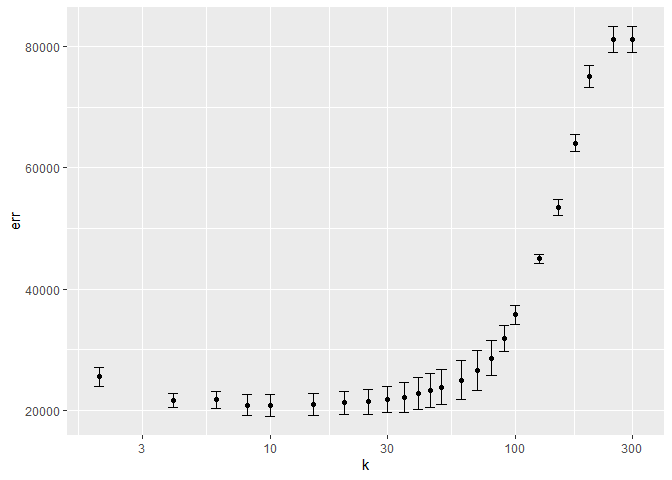
\includegraphics{Homework-1_files/figure-latex/unnamed-chunk-12-1.pdf}

\begin{Shaded}
\begin{Highlighting}[]
\NormalTok{knn13 }\OtherTok{=} \FunctionTok{knnreg}\NormalTok{(price }\SpecialCharTok{\textasciitilde{}}\NormalTok{ mileage, }\AttributeTok{data=}\NormalTok{sclass\_65AMG\_train, }\AttributeTok{k=}\DecValTok{13}\NormalTok{)}
\FunctionTok{rmse}\NormalTok{(knn13, sclass\_65AMG\_test)}
\end{Highlighting}
\end{Shaded}

\begin{verbatim}
## [1] 22909.13
\end{verbatim}

\begin{Shaded}
\begin{Highlighting}[]
\NormalTok{sclass\_65AMG\_test }\OtherTok{=}\NormalTok{ sclass\_65AMG\_test }\SpecialCharTok{\%\textgreater{}\%}
  \FunctionTok{mutate}\NormalTok{(}\AttributeTok{price\_pred =} \FunctionTok{predict}\NormalTok{(knn13, sclass\_65AMG\_test))}

\NormalTok{p\_test }\OtherTok{=} \FunctionTok{ggplot}\NormalTok{(}\AttributeTok{data =}\NormalTok{ sclass\_65AMG\_test) }\SpecialCharTok{+} \FunctionTok{geom\_point}\NormalTok{(}\AttributeTok{mapping =} \FunctionTok{aes}\NormalTok{(}\AttributeTok{x=}\NormalTok{mileage, }\AttributeTok{y=}\NormalTok{price), }\AttributeTok{alpha =} \FloatTok{0.8}\NormalTok{) }\SpecialCharTok{+} \FunctionTok{ylim}\NormalTok{(}\DecValTok{7000}\NormalTok{, }\DecValTok{20000}\NormalTok{)}
\NormalTok{p\_test}
\end{Highlighting}
\end{Shaded}

\begin{verbatim}
## Warning: Removed 59 rows containing missing values (geom_point).
\end{verbatim}

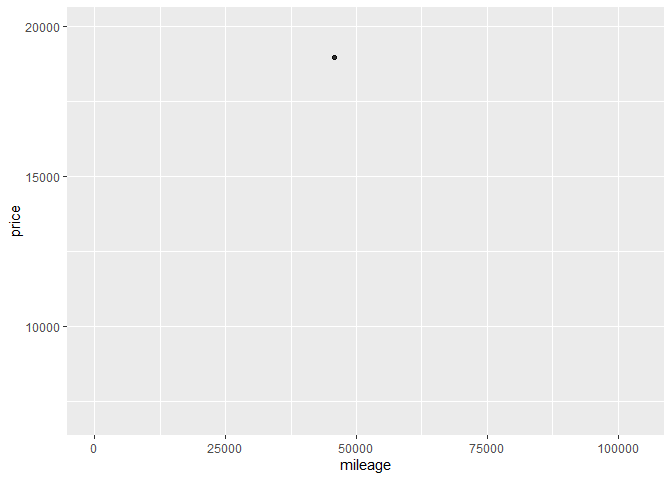
\includegraphics{Homework-1_files/figure-latex/unnamed-chunk-12-2.pdf}

\begin{Shaded}
\begin{Highlighting}[]
\NormalTok{p\_test }\SpecialCharTok{+} \FunctionTok{geom\_line}\NormalTok{(}\FunctionTok{aes}\NormalTok{(}\AttributeTok{x=}\NormalTok{mileage, }\AttributeTok{y=}\NormalTok{price\_pred), }\AttributeTok{color=}\StringTok{\textquotesingle{}green\textquotesingle{}}\NormalTok{, }\AttributeTok{size=}\FloatTok{1.5}\NormalTok{)}
\end{Highlighting}
\end{Shaded}

\begin{verbatim}
## Warning: Removed 59 rows containing missing values (geom_point).
\end{verbatim}

\begin{verbatim}
## Warning: Removed 59 row(s) containing missing values (geom_path).
\end{verbatim}

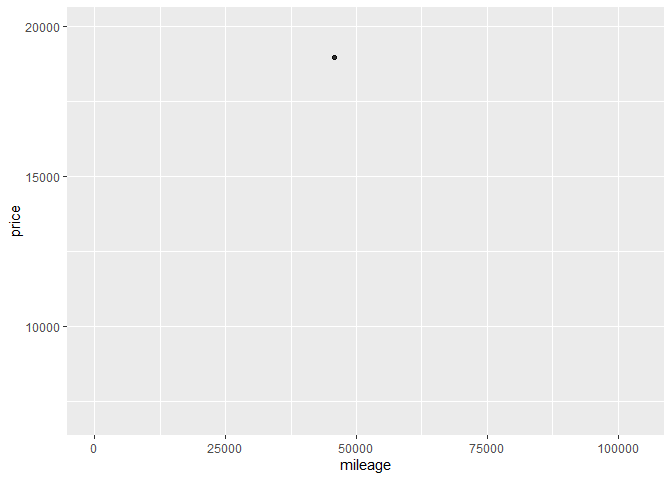
\includegraphics{Homework-1_files/figure-latex/unnamed-chunk-12-3.pdf}

\end{document}
